\documentclass[11pt, a4paper]{article}
\usepackage[norsk]{babel}

%For strikethrough
%\usepackage{ulem}

%For landscpe orientation \begin{landscape}...
\usepackage{pdflscape}
\newcommand{\blandscape}{\begin{landscape}}
\newcommand{\elandscape}{\end{landscape}}

%For rotating a figure \begin{sidewaysfigure}...
\usepackage{rotating}
\newcommand{\brotatefig}{\begin{sidewaysfigure}}
\newcommand{\erotatefig}{\end{sidewaysfigure}}


%
%To fix CLSreferenses bug
%This will probably have to be updated when using later rmarkdown and or pandoc versions


%For fill text
\usepackage{blindtext}

%For equations
\usepackage{amsmath}
%\savesymbol{medspace}
%\usepackage{txfonts}

%for tables spanning pages
\usepackage{longtable}

%Force floats to appear after text
%\usepackage{flafter}



%For linenumbers

%For references
%\usepackage{natbib} %%Handled by pandoc!
%\bibliographystyle{nina}
\usepackage[hidelinks,
            pdfborder={0 0 0},
            colorlinks = true,
            linkcolor = black,
            urlcolor = darkblue,
            pdfauthor={
                          Skriv in forfatter her
                                       ,~Skriv in forfatter her
                           ,~Skriv in forfatter her
                                       ,~Skriv in siste forfatter her
                         },
            pdftitle={Skriv in titell nivå 1 her},
            pdfsubject={Skriv in titell nivå 2 her},
            pdfkeywords={
                            geografisk område (land, fylke, kommune),~
                            art (fauna, flora, høyere taksonomisk
enhet,~
                            konsekvensutredning,~
                            overvåkingsrapport,~
                            etterundersøkelse,~
                            vassdrag,~
                            økosystemtjenester,~
                            radioaktivitet,~
                          }]{hyperref}


%For getting total pagecount
\usepackage{lastpage}

%For typesetting of bullet lists
\providecommand{\tightlist}{%
  \setlength{\itemsep}{0pt}\setlength{\parskip}{0pt}}

%To get pdf production date in proper format
\usepackage[norsk]{datetime}
\newdateformat{ninadate}{%
\monthname[\THEMONTH]~ \THEYEAR}

%Set fonts
%Note that we need to suppress ligaturs to mimic standard windows behaviour with Calibri
\usepackage{fontspec}
\defaultfontfeatures{Ligatures={NoRequired, NoCommon, NoContextual}}
\setmainfont{Calibri}
\newfontfamily{\narrow}{Calibri}
\newfontfamily{\narrowbold}{Calibri Bold}
\newfontfamily{\arialnarrow}{Arial Narrow}
\newfontfamily{\arialnarrowbold}{Arial Narrow Bold}
%\restoresymbol{fontspec}{medspace}


%To insert manual hyphens
\usepackage{hyphenat}

%To set caption font
%\usepackage[font=it,labelfont=bf]{caption}
\usepackage[font=it,format=plain,labelfont=bf,justification=justified,singlelinecheck=false,labelsep=period]{caption}

%Modify defaults to restrict the floating of figures
\renewcommand{\topfraction}{.85}
\renewcommand{\bottomfraction}{.7}
\renewcommand{\textfraction}{.15}
\renewcommand{\floatpagefraction}{.66}
\setcounter{topnumber}{3}
\setcounter{bottomnumber}{3}
\setcounter{totalnumber}{4}

%To place table caption above table
\usepackage{float}
\floatstyle{plaintop}
\restylefloat{table}
\setlength{\belowcaptionskip}{3mm}

%To refer to sections, figures and tables
\usepackage{nameref}
\newcommand*{\myref}[1]{\hyperref[{#1}]{\autoref*{#1} \nameref*{#1}}}
%Define own http_links to get underline links
\usepackage{soul}
\setul{.2ex}{.15ex}
\renewcommand*{\href}[2]{\hyperref[#1]{\color{darkblue}\setulcolor{darkblue}\ul{\mbox{#2}}}}
%\renewcommand*{\href}[1]{\hyperref[#1]{\color{darkblue}\setulcolor{darkblue}\ul{\mbox{#1}}}}


%Modify table of contents style
%\usepackage{titlesec}
\usepackage{titletoc}
\setcounter{tocdepth}{4}
%\contentsmargin{2.3em}
\contentsmargin{0em}
%\dottedcontents{section}[2.3em]{\bfseries}{1.3em}{5pt}
\dottedcontents{section}[1.3em]{\bfseries}{1.3em}{5pt}
\dottedcontents{subsection}[4.1em]{}{2.9em}{5pt}
\dottedcontents{subsubsection}[6.6em]{}{2.9em}{5pt}
\dottedcontents{paragraph}[10.2em]{}{3.6em}{5pt} %%too wide dots
\usepackage{setspace}

%To adjust margins and use left justification
\usepackage[a4paper, left=1.5cm,right=3.5cm,top=2cm,bottom=2cm,headheight=1cm]{geometry}
%\usepackage[document]{ragged2e}

%To adjust heading spacings
\usepackage{titlesec}
%To fix bug in titlesec 2.10.1 - that prevented section numbering
\usepackage{etoolbox}
\makeatletter
\patchcmd{\ttlh@hang}{\parindent\z@}{\parindent\z@\leavevmode}{}{}
\patchcmd{\ttlh@hang}{\noindent}{}{}{}
\makeatother
%end fix bug
\titlespacing{\subsection}{0pt}{12pt plus 4pt minus 2pt}{0pt plus 2pt minus 2pt}
\titlespacing{\subsubsection}{0pt}{12pt plus 4pt minus 2pt}{0pt plus 2pt minus 2pt}
\titleformat{\paragraph}
{\normalfont\normalsize\bfseries}{\theparagraph}{1em}{}
\titlespacing*{\paragraph}{0pt}{12pt plus 4pt minus 2pt}{0pt plus 2pt minus 2pt}

\newcommand{\smallspace}{\vspace{3mm}}
%\newcommand{\medspace}{\vspace{5mm}}

%Adjust paragraph indentations
\setlength{\parindent}{0pt}

%To adjust graphics
\usepackage{graphicx}
%\usepackage{epstopdf}

\usepackage{tikz}
\usetikzlibrary{positioning}
\usepackage{xstring}
\usepackage{forloop}


%Modify headers and footers
\usepackage{fancyhdr}
\newsavebox{\myheadbox}
\pagestyle{fancy}
\addtolength{\headheight}{2pt}
\renewcommand{\headrulewidth}{0pt}
\renewcommand{\footrulewidth}{0pt}

%Defines the line in the pagefooter
\newcommand*\ruleline[1]{\par\noindent\raisebox{.4ex}{\makebox[\linewidth]{\hrulefill\hspace{1ex}\raisebox{-.4ex}{#1}\hspace{1ex}\hrulefill}}}

%Define titlepage footer
\usepackage{tikzpagenodes}
\fancypagestyle{titlefooter}{% Define title footer (change to svg logo)
  \fancyhf{}
  \begin{center}
  \vspace{-1.2cm}
  \Large\shadOrange{\narrow{\textbf{www.nina.no}}}
  \vspace{.2cm}
  \end{center}
  \begin{tikzpicture}[remember picture,overlay]
    \node (a) at (-4,-1.68) {};
    \node (b) at (0.37,-8.12) {};
    \coordinate[above=2.5cm of b,xshift=-.6cm]  (legend);
    \coordinate[below=.49cm of a,xshift=3.3cm]  (rapportnr);
    \fill[footgrey] (a) rectangle (b);
    \node[rotate=90] at (legend) {\color{darkgrey}\Huge{\arialnarrowbold{NINA~}\arialnarrow{Rapport}}};
    \node at (rapportnr) {\color{orange}\Huge{\narrowbold{1234}}};
 \end{tikzpicture}
\lfoot{\vspace{1.25cm}\hspace{-1.45cm}
\includegraphics[height=1.6cm]{logo.eps}}
\rfoot{\vspace{2.4cm}\Large\color{darkgrey}{\arialnarrow{Norsk institutt for naturforskning~~~}}}
\begin{tikzpicture}[remember picture,overlay]
  \fill[footgrey]
    (current page.south west)
    rectangle
  (current page.east|-current page footer area.south east);
  \end{tikzpicture}
}

 \usepackage{tikzpagenodes}


% one way of including bg-pic
% \usepackage{eso-pic}
% \newcommand\BackgroundPic{%
% \put(0,0){%
% \parbox[b][\paperheight]{\paperwidth}{%
% \vfill
% \centering
% \includegraphics[width=\paperwidth,height=\paperheight,%
% keepaspectratio]{title_page_bg.png}%
% \vfill
% }}}

%Define endpage footer
\fancypagestyle{endfooter}{% Define endpage footer (change to svg logo)

  \fancyhf{}
  \fancyfootoffset[R]{0cm}
  \begin{center}
    \vspace{-1.2cm}
    \Large\shadOrange{\narrow{\textbf{www.nina.no}}}

 \begin{tikzpicture}[remember picture,overlay]
 \node (a) at (11.05, 4.3) {};
 \node (b) at (15,-2.1) {};
 \coordinate[above=2.5cm of b,xshift=-3cm]  (legend);
 \coordinate[below=.5cm of a,xshift=1cm]  (rapportnr);
 \fill[footgrey] (a) rectangle (b);
 \node[rotate=90] at (legend) {\color{darkgrey}\Huge{\arialnarrowbold{NINA~}\arialnarrow{Rapport}}};
 \node at (rapportnr) {\color{orange}\huge{\narrowbold{1234}}};
\end{tikzpicture}
    \begin{minipage}{0.386\linewidth}
    {\begin{flushleft}\color{darkgrey}\vspace{1.2cm}\large\narrow\em{\textbf{Norsk institutt for naturforskning, NINA,} er en uavhengig stiftelse som forsker på natur og samspillet natursammfunn.

    \bigskip
    NINA ble etablert i 1988. Hovedkontoret er i Trondheim, med avdelingskontorer i Tromsø, Lillehammer, Bergen og Oslo. I tillegg driver NINA Sæterfjellet avlsstasjon for fjellrev på Oppdal, og forskningsstasjonen for vill laksefisk på Ims i Rogaland.

    \bigskip
    NINAs virksomhet omfatter både forskning og utredning, miljøoveråking, rådgivning og evaluering. NINA har stor bredde i kompetanse og erfaring med både naturvitere og samfunnsvitere i staben. Vi har kunnskap om artene, naturtypene, sammfunnets bruk av naturen og sammenhenger med de store drivkreftene i naturen.} \end{flushleft}}
    \end{minipage}
    \vspace{3cm}
    \vfill{}{\normalsize{ISSN: 1504-3312 \\
  ISBN: 978-82-426-1234-5}}
  \end{center}
  \lfoot{\color{darkgrey}\vspace{0.5cm}\Large\narrow{\textbf{Norsk institutt for naturforskning}}\\
\begingroup
\narrow
\normalsize NINA Hovedkontor\\
Postadresse: Postboks 5685 Torgarden, 7485 Trondheim\\
Besøks-/leveringsadresse: Høgskoleringen 9, 7034 Trondheim\\
Telefon: 73 80 14 00, Telefaks: 73 80 14 01\\
E-post: firmapost@nina.no\\
Organisasjonsnummer 9500 37 687\\
http://www.nina.no
\endgroup}
  % \rfoot{\vspace{2cm}\hspace{-3cm}
\includegraphics[height=1.6cm]{logo.eps}\\
  % \Large\darkGrey{\narrow{Samarbeid og kunnskap for framtidas miljøløsninger}}
  % }
  \rfoot{\vspace{2.3cm}\savebox{\myheadbox}{\Large\darkGrey{\narrow{Samarbeid og kunnskap for framtidas miljøløsninger}}}\makebox[\wd\myheadbox][c]{
\includegraphics[height=1.6cm]{logo.eps}}\\\usebox{\myheadbox}}

    \begin{tikzpicture}[remember picture,overlay]
  \fill[footgrey]
    (current page.south west)
    %(current page.west|-current page footer area.north west)
    rectangle
  (current page.east|-current page footer area.north east);
  %(current page text area.south west);
  \end{tikzpicture}

%  \tikz[remember picture,overlay] {%
%  \draw [blue,line width=2mm]
%  (current page.south west)
%  rectangle
%  (current page.north east)
%  ;
%  \draw [green]
%  (current page text area.south west)
%  rectangle
%  (current page text area.north east)
%  ;
%  \draw [yellow]
%  (current page marginpar area.south west)
%  rectangle
%  (current page marginpar area.north east)
%  ;
%  \draw [red]
%  (current page header area.south west)
%  rectangle
%  (current page header area.north east)
%  ;
%  \draw [orange]
%  (current page footer area.south west)
% rectangle
%  (current page footer area.north east)
%  ;
%  }%

}

%Make sure it always produce even numbered document (adding empty page if necessary)
\usepackage{scrextend}
\newcommand{\OpenNewPageIfNeeded}{%
  \Ifthispageodd{\fancyhf{}\newgeometry{bottom=6.6cm, top=2cm, left=1.5cm, right=1.5cm, headsep=0cm, footskip=0.5cm}\null\clearpage~\pagestyle{endfooter}
  }{\fancyhf{}\newgeometry{bottom=6.6cm, top=2cm, left=1.5cm, right=1.5cm, headsep=0cm, footskip=0.5cm}\null\pagestyle{endfooter}}
}
\AtEndDocument{\OpenNewPageIfNeeded}


%Define custom code background shading
\definecolor{shadecolor}{RGB}{238,238,238}


%Set up custom colors
\usepackage{xcolor}
\usepackage{blindtext}
\definecolor{darkOrange}{RGB}{245,127, 0}
\definecolor{lightOrange}{RGB}{219,140, 68}
\definecolor{ashgrey}{RGB}{128, 128, 128}
\definecolor{darkgrey}{RGB}{66, 85, 99}
\definecolor{footgrey}{RGB}{212, 215, 221}
\definecolor{darkblue}{RGB}{0, 79, 113}

\newcommand{\shadOrange}[1]{\textcolor{lightOrange}{#1}}
\newcommand{\orange}[1]{\textcolor{darkOrange}{#1}}
\newcommand{\lightGrey}[1]{\textcolor{ashgrey}{#1}}
\newcommand{\darkGrey}[1]{\textcolor{darkgrey}{#1}}

\begin{document}
%\AddToShipoutPicture*{\BackgroundPic}

\newgeometry{bottom=6cm, top=4.6cm, left=3.48cm, right=1.5cm}

\begin{titlepage}
%Testing out title page bg-pic
\thispagestyle{titlefooter}

%Testing out tikz title page bg-pic
% \begin{tikzpicture}[remember picture,overlay, anchor=south west]
%   \node at (current page.south west){\includegraphics[width=\paperwidth,height=\paperheight,%
%  keepaspectratio]{title_page_bg.png}};
% \end{tikzpicture}

\huge{Skriv in titell nivå 1 her} \par\vspace{.3cm}
\LARGE{Skriv in titell nivå 2 her} \par\vspace{.6cm}
\hspace{0cm}\Large{Skriv in forfatter her},
\hspace{-2mm}~\Large{Skriv in forfatter her},
\hspace{-2mm}~\Large{Skriv in forfatter her},
\hspace{-2mm}~\Large{Skriv in siste forfatter her}

\begin{tikzpicture}[remember picture,overlay, anchor=south west]
  \node at ([yshift=4.77cm,xshift=-0.24cm]current page.south west){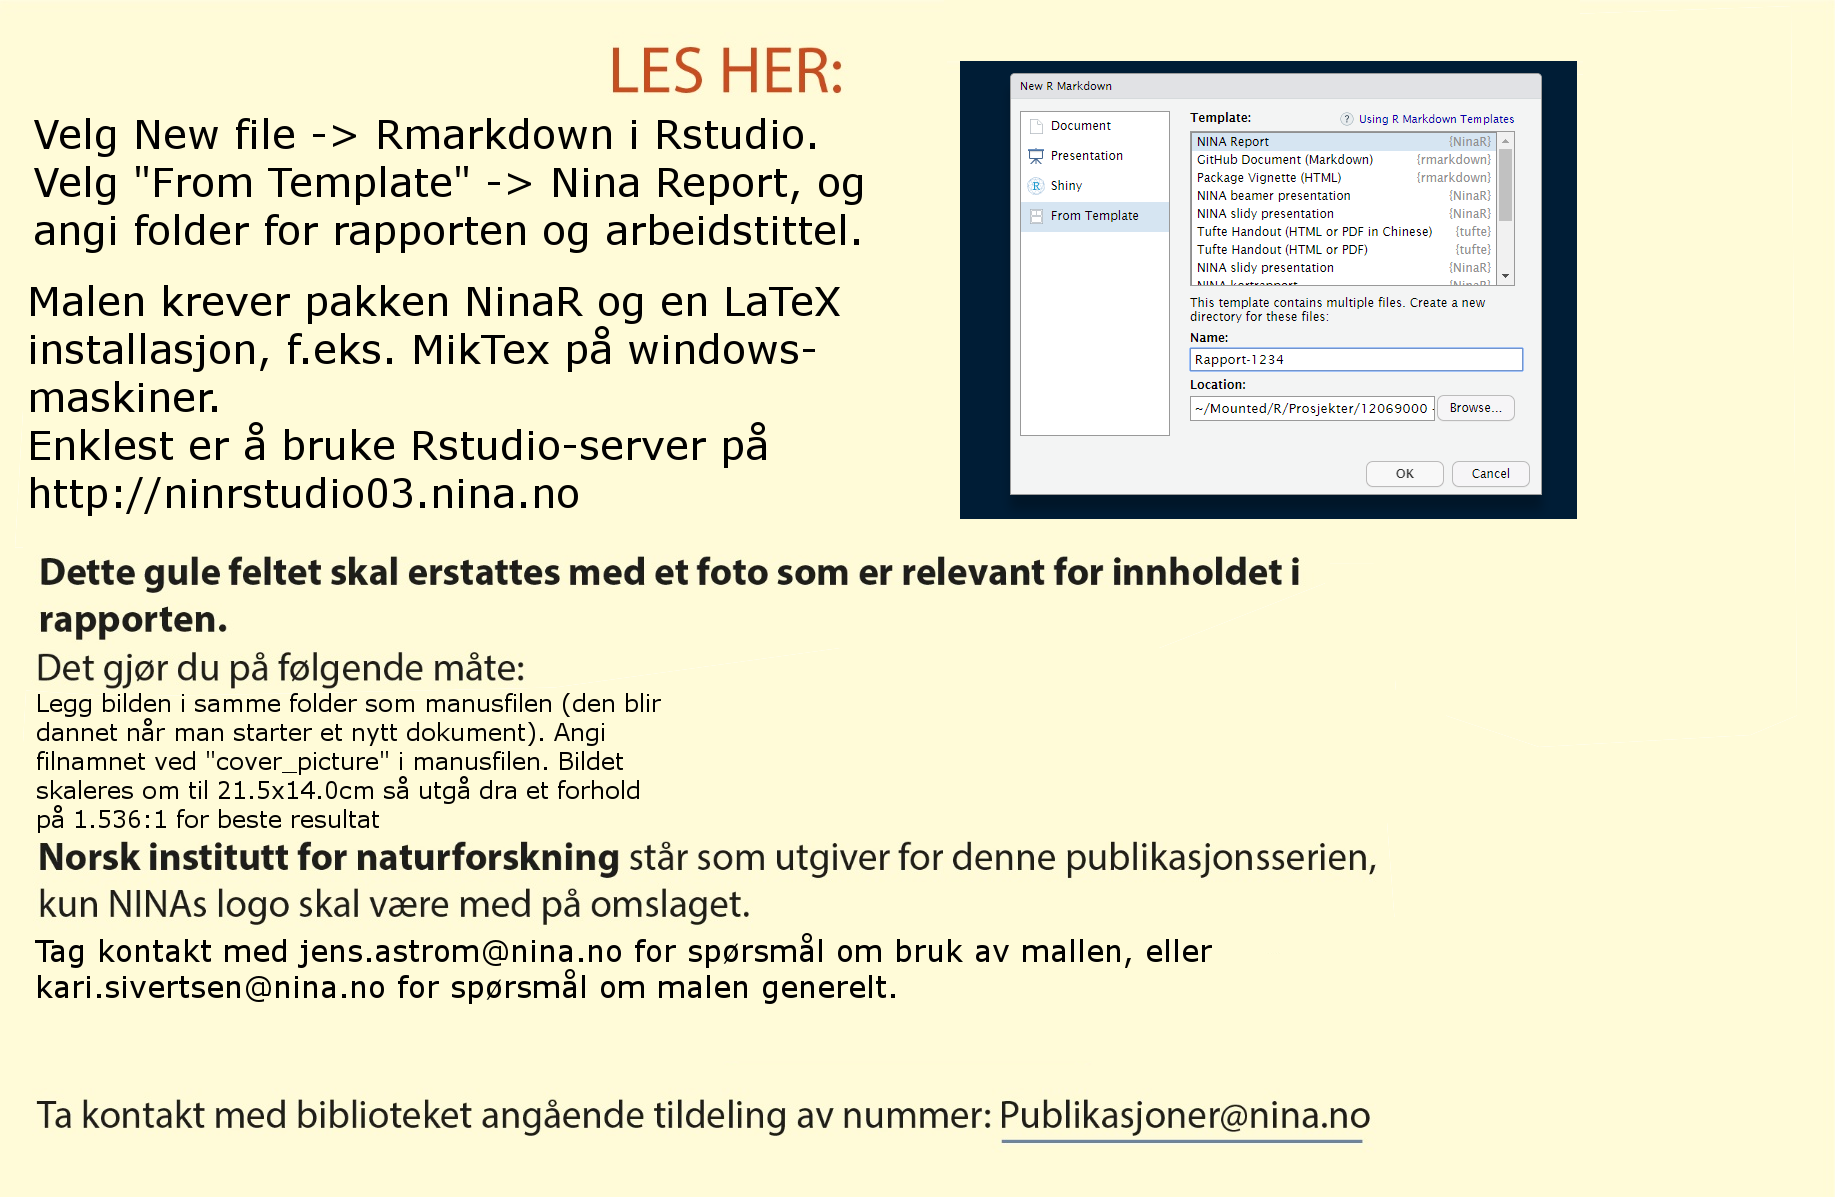
\includegraphics[width=21.35cm, height=13.9cm]{coverPicture.png}};
 \end{tikzpicture}
\restoregeometry
\end{titlepage}
\newgeometry{bottom=3cm, top=3cm, left=2.68cm, right=2.68cm}
%Second page
\cfoot{}

\section*{\narrow{NINAs publikasjoner}}
\hspace{1ex}

\subsection*{\small{NINA Rapport}}
{\normalsize Dette er NINAs ordinære rapportering til oppdragsgiver etter gjennomført forsknings\hyp{}, overvåkings\hyp{} eller utredningsarbeid. I tillegg vil serien favne mye av instituttets øvrige rapportering, for eksempel fra seminarer og konferanser, resultater av eget forsknings\hyp{} og utredningsarbeid og litteraturstudier. NINA Rapport kan også utgis på engelsk, som NINA Report.
}

\subsection*{\small{NINA Temahefte}}
{\normalsize Heftene utarbeides etter behov og serien favner svært vidt; fra systematiske bestemmelsesnøkler til informasjon om viktige problemstillinger i samfunnet. Heftene har vanligvis en populærvitenskapelig form med vekt på illustrasjoner. NINA Temahefte kan også utgis på engelsk, som NINA Special Report.}

\subsection*{\small{NINA Fakta}}
{\normalsize Faktaarkene har som mål å gjøre NINAs forskningsresultater raskt og enkelt tilgjengelig for et større
publikum. Faktaarkene gir en kort framstilling av noen av våre viktigste forskningstema.}

\subsection*{\small{Annen publisering}}
{\normalsize I tillegg til rapporteringen i NINAs egne serier publiserer instituttets ansatte en stor del av sine forsk- ningsresultater i internasjonale vitenskapelige journaler og i populærfaglige bøker og tidsskrifter.}

\subsection*{\small{NINA Map}}
{\normalsize Rik metadata om en modellutgang som produserer et geografisk kartresultat.}
\clearpage
\newgeometry{bottom=3cm, top=3cm, left=2.68cm, right=2.68cm}
%Page 3
\setcounter{page}{1}
\fancyfoot[C]{
\newgeometry{bottom=3cm, top=3cm, left=2.68cm, right=2cm}
\vspace{-0.5cm}\hfill\Large{\narrowbold{Norsk institutt for naturforskning}}}
\vspace{2cm}

\huge{Skriv in titell nivå 1 her} \par\vspace{.5cm}
\LARGE{Skriv in titell nivå 2 her} \par\vspace{1cm}
\hspace{0cm}\LARGE{Skriv in forfatter her} \par
\LARGE{Skriv in forfatter her} \par
\LARGE{Skriv in forfatter her} \par
\LARGE{Skriv in siste forfatter her} \par

\clearpage
\newgeometry{bottom=2.5cm, top=2.5cm, left=2.5cm, right=2.5cm}
%Page 4
\fancyhf{}
\pagestyle{fancy}
\fancyfoot[c]{\ruleline{\thepage}}
\fancyhead[c]{\ruleline{\tiny{NINA Rapport 1234}}}
% To count also the first page (for new template)
\addtocounter{page}{1}

\normalsize
\newgeometry{bottom=3cm, top=2.6cm, left=2.82cm, right=6.2cm}
\small{Brum, O., Robin, K. 2016. En veldig bra
titel.}~NINA Rapport 1234. Norsk institutt for naturforskning. \par \href{http://hdl.handle.net/11250/fås
av bibliotek}{http://hdl.handle.net/11250/fås av
bibliotek} \par \smallspace
Trondheim, \ninadate\today \par \smallspace
ISSN: 1504-3312 \par
ISBN: 978-82-426-1234-5 \par  \smallspace
{\scriptsize{RETTIGHETSHAVER}} \par
© Norsk institutt for naturforskning  \par
Denne rapporten er lisensiert under Creative Commons Navngivelse 4.0 \par
Internasjonal lisens: \href{https://creativecommons.org/licenses/by/4.0/}{Creative Commons — Attribution 4.0 International — CC BY 4.0}\par \smallspace
{\scriptsize{TILGJENGELIGHET}} \par
Åpen \par \smallspace
{\scriptsize{PUBLISERINGSTYPE}} \par
Digitalt dokument (pdf) \par \smallspace
{\scriptsize{KVALITETSSIKRET AV}} \par
xx \par \smallspace
{\scriptsize{ANSVARLIG SIGNATUR}} \par
Forskningssjef Forskningssjef {[}fylles ut av forskningssjefen{]}
(sign.) \par \smallspace
{\scriptsize{OPPDRAGSGIVER(E)/BIDRAGSYTER(E)}} \par
xx \par \smallspace
{\scriptsize{OPPDRAGSGIVERS REFERANSE}} \par
xx \par \smallspace
{\scriptsize{KONTAKTPERSON(ER) HOS OPPDRAGSGIVER/BIDRAGSYTER}} \par
xx \par \smallspace
{\scriptsize{FORSIDEBILDE}} \par
Forsidebildetekst~ \copyright~ Fotografnavn \par \smallspace
{\scriptsize{NØKKELORD}} \par\smallskip
\small{\hyp{} geografisk område (land, fylke, kommune)} \par
\small{\hyp{} art (fauna, flora, høyere taksonomisk enhet} \par
\small{\hyp{} konsekvensutredning} \par
\small{\hyp{} overvåkingsrapport} \par
\small{\hyp{} etterundersøkelse} \par
\small{\hyp{} vassdrag} \par
\small{\hyp{} økosystemtjenester} \par
\small{\hyp{} radioaktivitet} \par
\vspace{5mm}
{\scriptsize{KEY WORDS}} \par\smallskip
\small{\hyp{} se nøkkelord} \par

\vfill
%\noindent


\begin{minipage}{\linewidth}
\scriptsize{KONTAKTOPPLYSNINGER} \par\smallspace
\scriptsize
\leavevmode\hbox to \linewidth{%
\hspace{-.25cm}
\begin{tabular}[t]{l@{}}
\textbf{NINA hovedkontor} \\
Postboks 5685 Torgarden\\
7485 Trondheim\\
Telefon: 73 80 14 00
\end{tabular}
\hfill
\begin{tabular}[t]{l@{}}
\textbf{NINA Oslo} \\
Sognsveien 68 \\
0855 Oslo \\
Telefon: 73 80 14 00
\end{tabular}%
\hfill
\begin{tabular}[t]{l@{}}
\textbf{NINA Tromsø} \\
Postboks 6606 Langnes \\
9296 Tromsø \\
Telefon: 77 75 04 00
\end{tabular}%
\hfill
\begin{tabular}[t]{l@{}}
\textbf{NINA Lillehammer} \\
Vormstuguvegen 40 \\
2624 Lillehammer \\
Telefon: 73 80 14 00
\end{tabular}%
\begin{tabular}[t]{l@{}}
\textbf{NINA Bergen} \\
Thormøhlensgate 55 \\
5006 Bergen \\
Telefon: 73 80 14 00
\end{tabular}%
}
\par\vspace{3mm}
www.nina.no
\vspace{-4mm}
\end{minipage}

\clearpage
\setcounter{secnumdepth}{0}
\newgeometry{bottom=3cm, top=3cm, left=2.68cm, right=2.68cm}
\section{Sammendrag}
\normalsize{Brum, O., Robin, K. 2016. En veldig bra
titel.} NINA Rapport 1234. Norsk institutt for naturforskning. \par\href{http://hdl.handle.net/11250/fås
av bibliotek}{http://hdl.handle.net/11250/fås av bibliotek} \par
\vspace{0.5cm}
\normalsize{
Tekst inn her, et kort resymé av innholdet.} \\

\vspace{1cm}
\small
Skriv in forfatter her, Author adress, for.efternavn@nina.no  \par
Skriv in forfatter her, Author adress, for.efternavn@nina.no  \par
Skriv in forfatter her, Author adress, for.efternavn@nina.no  \par
Skriv in siste forfatter her, Author adress, for.efternavn@nina.no  \par
\normalsize
\clearpage

\setcounter{secnumdepth}{0}
\section{Preamble}
\small{the Poo, W., Robin, C. 2016. A very good
title.} NINA Rapport 1234. Norsk institutt for naturforskning. \par\href{http://hdl.handle.net/11250/fås
av bibliotek}{http://hdl.handle.net/11250/fås av bibliotek}\par
\vspace{0.5cm}
\normalsize{
This document describes for maps of distributions\ldots Using the
`Usage, Overview, Data, Model, Assessment, and Prediction' (UODMAP)
protocol.} \\

\vspace{1cm}
\small
Skriv in forfatter her, Author adress, for.efternavn@nina.no  \par
Skriv in forfatter her, Author adress, for.efternavn@nina.no  \par
Skriv in forfatter her, Author adress, for.efternavn@nina.no  \par
Skriv in siste forfatter her, Author adress, for.efternavn@nina.no  \par
\normalsize
\clearpage

\setcounter{secnumdepth}{0}
\section{Useage Or Application}
\normalsize{
Usage or Application} \\
\normalsize
\clearpage


\doublespacing
\tableofcontents
\addcontentsline{toc}{section}{Innhold}
\singlespacing
\clearpage

\section{Forord}

\normalsize
Forord inn her\par
\medskip
Stedforord, \par
\medskip
Prosjektleder



\clearpage
\setcounter{secnumdepth}{4}
\setlength{\parskip}{6pt}

\hypertarget{overview}{%
\subsection{Overview}\label{overview}}

\hypertarget{model-objective}{%
\subsubsection{Model objective}\label{model-objective}}

\emph{Model objective:}

\emph{Target output:}

\hypertarget{taxon-location-predictors-scale}{%
\subsubsection{Taxon, location, predictors,
scale}\label{taxon-location-predictors-scale}}

\textbf{Taxon}

\emph{Focal Taxon:}

\textbf{Location}

\emph{Location:}

\textbf{Scale of Analysis}

\emph{Spatial extent:} bounding box

\emph{Spatial resolution:}

\emph{Temporal extent:}

\emph{Boundary:}

\textbf{Biodiversity data}

\emph{Observation type:}

\emph{Response data type:}

\textbf{Predictors}

\emph{Predictor types:}

\hypertarget{conceptual-underpinning}{%
\subsubsection{Conceptual underpinning}\label{conceptual-underpinning}}

\textbf{Hypotheses}

\emph{Hypotheses:}

\textbf{Assumptions}

\emph{Model assumptions:}

\hypertarget{software-codes-and-data-availability}{%
\subsubsection{Software, codes and data
availability}\label{software-codes-and-data-availability}}

\textbf{Algorithms}

\emph{Modelling techniques:}

\emph{Model complexity:}

\emph{Model averaging:}

\textbf{Workflow}

\emph{Model workflow:}

\begin{enumerate}
\def\labelenumi{\arabic{enumi}.}
\tightlist
\item
\item
\item
  4\ldots.
\end{enumerate}

\textbf{Software}

\emph{Software:}

\emph{Data availability:}

\hypertarget{data}{%
\subsection{Data}\label{data}}

\hypertarget{biodiversity-data}{%
\subsubsection{Biodiversity data}\label{biodiversity-data}}

\emph{Taxon names:}

\emph{Ecological level:}

\emph{Data sources:}

\emph{Sample size:}

\hypertarget{data-partitioning}{%
\subsubsection{Data partitioning}\label{data-partitioning}}

\emph{Training data:}

\emph{Validation data:}

\hypertarget{environmental-data}{%
\subsubsection{Environmental data}\label{environmental-data}}

\hypertarget{predictor-variables}{%
\paragraph{Predictor variables}\label{predictor-variables}}

\emph{Coordinate reference system:}

\hypertarget{topography}{%
\subparagraph{Topography}\label{topography}}

\hypertarget{soil}{%
\subparagraph{Soil}\label{soil}}

\hypertarget{climate}{%
\subparagraph{Climate}\label{climate}}

\hypertarget{transfer-data}{%
\paragraph{Transfer data}\label{transfer-data}}

\hypertarget{climate-1}{%
\subparagraph{Climate}\label{climate-1}}

\hypertarget{forest-cover-and-type}{%
\subparagraph{Forest cover and type}\label{forest-cover-and-type}}

\hypertarget{model}{%
\subsection{Model}\label{model}}

\hypertarget{habitat-suitability-model-hsm}{%
\subsubsection{Habitat Suitability Model
(HSM)}\label{habitat-suitability-model-hsm}}

\hypertarget{variable-selection}{%
\paragraph{Variable selection}\label{variable-selection}}

\hypertarget{model-setting-and-model-complexity}{%
\paragraph{Model setting and model
complexity}\label{model-setting-and-model-complexity}}

\hypertarget{model-estimates-variable-importance}{%
\paragraph{Model estimates, variable
importance}\label{model-estimates-variable-importance}}

\emph{Variable importance:}

\hypertarget{model-selection-averaging-ensembles}{%
\paragraph{Model selection, averaging,
ensembles}\label{model-selection-averaging-ensembles}}

\emph{Model selection:} \emph{Model averaging:}

\hypertarget{non-independence-analyses}{%
\paragraph{Non-independence analyses}\label{non-independence-analyses}}

\hypertarget{threshold-selection}{%
\paragraph{Threshold selection}\label{threshold-selection}}

\hypertarget{movement-model}{%
\subsubsection{Movement Model}\label{movement-model}}

\hypertarget{connectivity-metrics-and-assessment}{%
\paragraph{Connectivity metrics and
assessment}\label{connectivity-metrics-and-assessment}}

\hypertarget{movement-flow}{%
\subparagraph{Movement flow}\label{movement-flow}}

\hypertarget{functional-connectivity}{%
\subparagraph{Functional connectivity}\label{functional-connectivity}}

\hypertarget{assessment}{%
\subsection{Assessment}\label{assessment}}

\hypertarget{preformance}{%
\subsubsection{Preformance}\label{preformance}}

\hypertarget{response-curves}{%
\subsubsection{Response curves}\label{response-curves}}

\hypertarget{prediction}{%
\subsection{Prediction}\label{prediction}}

\hypertarget{prediction-output}{%
\subsubsection{Prediction output}\label{prediction-output}}

\hypertarget{habitat-suitability}{%
\paragraph{Habitat suitability}\label{habitat-suitability}}

\emph{Prediction unit:}

\hypertarget{climate-vulnerability-index}{%
\paragraph{Climate vulnerability
index}\label{climate-vulnerability-index}}

\hypertarget{uncertainty-quantification}{%
\subsubsection{Uncertainty
quantification}\label{uncertainty-quantification}}

\hypertarget{discussion}{%
\subsection{Discussion}\label{discussion}}

\clearpage

\hypertarget{references}{%
\section{References}\label{references}}

\setlength{\parindent}{-0.2in}
\setlength{\parskip}{8pt}

\noindent


%\clearpage
%\fancyhf{}
%\newgeometry{a4paper, bottom=8cm, top=2cm, left=1.5cm, right=1.5cm}
%\pagestyle{endfooter}

\end{document}
